\subsection{Direccionamiento y decodificacióno}

\subsubsection{Construcción interna de una memoria}

La construcción interna de una memoria de acceso aleatorio de $m$ palabras y $n$ bits por palabra consta de $m \times n$ \textbf{celdas binarias de almacenamiento} y los correspondientes circuitos de decodificación que \textit{seleccionan palabras individuales}. La celda binaria de almacenamiento es el bloque de construcción básico de una unidad de memoria y es un circuito electrónico con entre cuatro y seis transistores. 

La celda binaria almacena un bit en su latch interno. La entrada de selección habilita a la celda para leer o escribir, y la entrada leer/escribir determina la operación de la celda. Un 1 en esa entrada hace que se efectúe la operación de lectura porque establece una trayectoria entre el latch y la terminal de salida. Un 0 en la entrada de leer/escribir hace que se efectúe la operación de escritura porque establece una trayectoria entre la terminal de entrada y el latch

Por ejemplo, una memoria que contiene palabras de $8$ bits, las celdas de almacenamiento de la memoria serian de manera ilutrativa como se muestra en la figura \ref{fig:memfoto2}.

\begin{figure}[h]
\centering
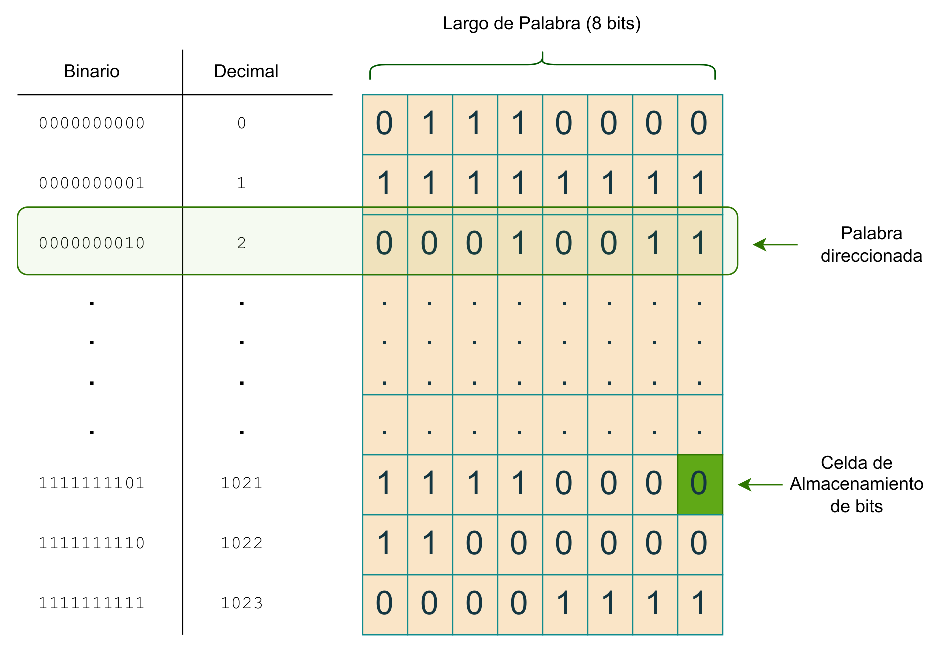
\includegraphics[scale=0.84]{img/memorias.eps}
\caption{Ejemplo de organización de una memoria de $1k$ x $8$}
\label{fig:memfoto2}
\end{figure}

\subsubsection{Selección de una palabra de memoria}
Para seleccionar una palabra de memoria, se requiere un decodificador que acepte la dirección de la palabra y abra las trayectorias necesarias para seleccionar la palabra especificada. La dirección de la palabra se aplica a las entradas del decodificador, y la salida correspondiente se activa. La salida activada se conecta a la línea de selección de palabra de memoria. La figura \ref{fig:memfoto3} se ilustra la construcción lógica de una RAM pequeña. Consta de cuatro palabras de cuatro bits cada una y tiene un total de 16 celdas binarias. Los pequeños bloques rotulados CB representan las celdas binarias con sus tres entradas y una salida. Una memoria de cuatro palabras necesita dos líneas de dirección. Las dos entradas de dirección pasan por un decodificador de $2 \times 4$ para seleccionar una de las cuatro palabras. El decodificador se habilita con la entrada de habilitar memoria. Si esa señal es 0, todas las salidas del decodificador son 0 y no se selecciona ninguna de las palabras de memoria. Si la señal es 1, se selecciona una de las cuatro palabras, especificada por el valor de las dos líneas de dirección. Una vez seleccionada una palabra, la entrada leer/escribir determina la operación. Durante la operación de lectura, los cuatro bits de la palabra seleccionada pasan por compuertas OR a las terminales de salida. Durante la operación de escritura, los datos disponibles en las líneas de entrada se transfieren a las cuatro celdas binarias de la palabra
seleccionada. Las celdas binarias que no están seleccionadas se inhabilitan, y sus valores binarios anteriores no cambian. Si la entrada de selección de memoria que llega al decodificador es 0, no se selecciona ninguna de las palabras y el contenido de todas las celdas permanece inalterado, sea cual sea el valor de la entrada leer/escribir.

\newpage
\begin{figure}[h]
\centering
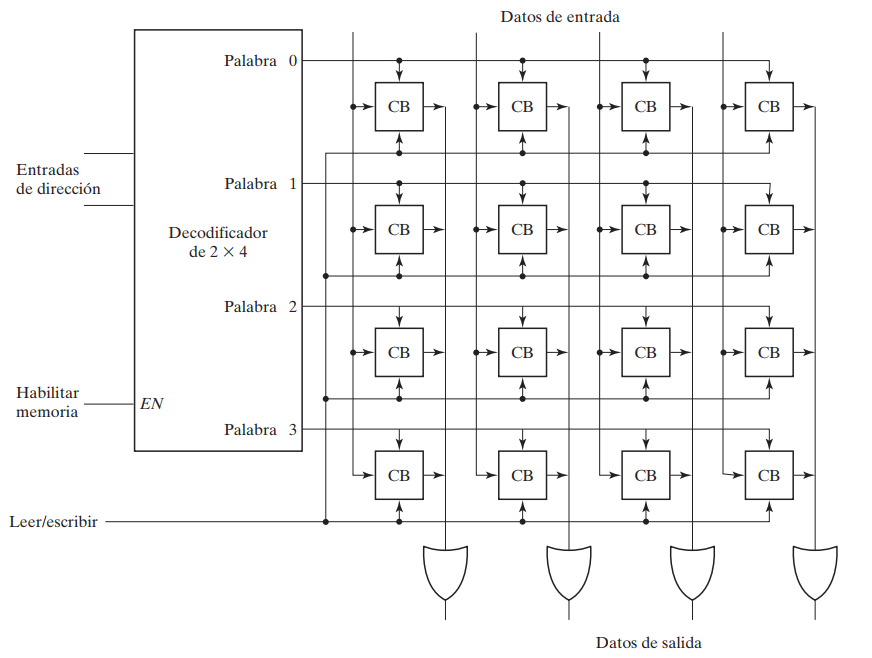
\includegraphics[scale=0.7]{img/selectdeco.png}
\caption{Diagrama de RAM $4 \times 6$}
\label{fig:memfoto3}
\end{figure}

\subsubsection{Decodificación bidiimensional}
La idea básica de la decodificación bidimensional es acomodar las celdas de memoria en un arreglo lo más cercano posible a un cuadrado. En esta configuración, se usan dos decodificadores con $k/2$ entradas cada uno, en vez de un decodificador con $k$ entradas. Un decodificador selecciona la fila y el otro selecciona la columna de una configuración de matriz bidimensional.

\begin{figure}[h]
\centering
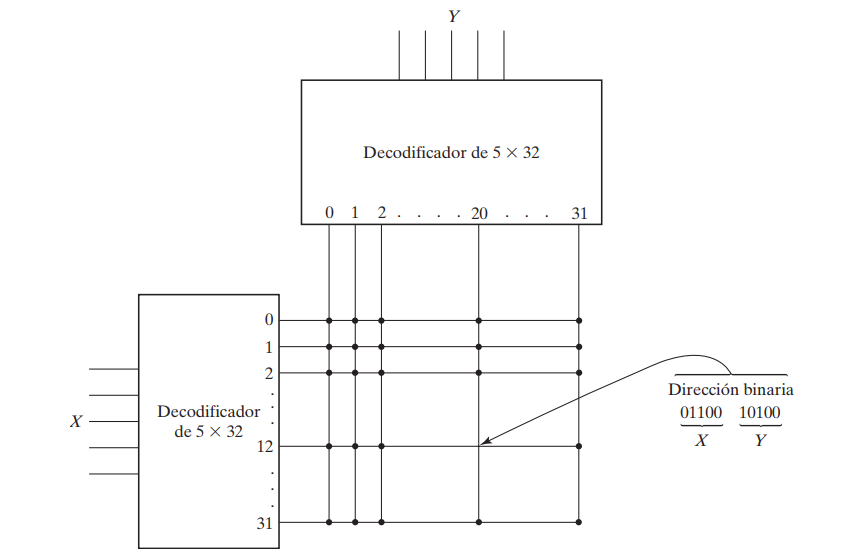
\includegraphics[scale=0.69]{img/decbi.png}
\caption{Decodificación bidimensional}
\label{fig:memfoto4}
\end{figure}

\subsection{Direccionamiento}
Una memoria de $1K \times 16$ tiene $10$ bits en la dirección y $16$ bits en cada palabra. La dirección de la memoria se especifica con $10$ bits, y cada dirección selecciona una palabra de $16$ bits. La primera dirección se especifica con $10$ ceros, y la última, con $10$ unos. Ello se debe a que $1023$ en binario es $1111111111$. Se selecciona una palabra de memoria por su dirección binaria. Cuando se lee o escribe una palabra, la memoria opera sobre los $16$ bits como una sola unidad.

\begin{mdframed}[backgroundcolor=gray!10,linewidth=0]
    Para generalizar, podriamos decir que una memoria de $m \times n$ tiene $m$ palabras y $n$ bits por palabra. La dirección de la memoria se especifica con $k$ bits, y cada dirección selecciona una palabra de $n$ bits. La primera dirección se especifica con $k$ ceros, y la última, con $k$ unos. Se selecciona una palabra de memoria por su dirección binaria. Cuando se lee o escribe una palabra, la memoria opera sobre los $n$ bits como una sola unidad.
\end{mdframed}

El bus de dirección es un conjunto de líneas que se usan para especificar la dirección de la palabra que se va a leer o escribir. El bus de datos es un conjunto de líneas que se usan para transferir información entre la memoria y el procesador. El bus de control es un conjunto de líneas que se usan para especificar la dirección de la transferencia de datos. La figura \ref{fig:memfoto5} muestra un diagrama de bloques de una memoria genérica.

\begin{figure}[h]
\centering
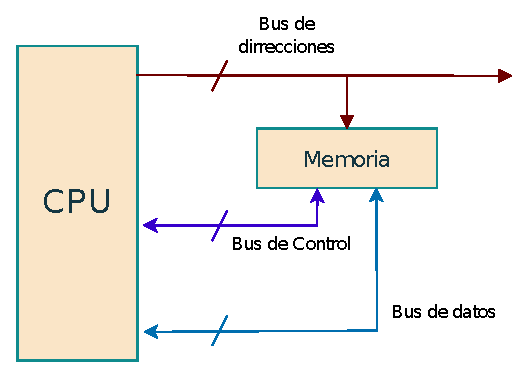
\includegraphics[scale=0.9]{img/buses.eps}
\caption{Diagrama de bloques de una memoria genérica}
\label{fig:memfoto5}
\end{figure}